\documentclass{beamer}

\usepackage[ngerman]{babel}
\usepackage{epstopdf}
\usepackage{bibgerm}
\usepackage[T1]{fontenc}
\usepackage[utf8]{inputenc}
\usepackage{ifthen}
\usepackage{graphicx}

\setbeamertemplate{navigation symbols}{}
\setbeamertemplate{footline}[frame number]

\title{Zwischenstand: Load Balancing DNS}
\author{Sebastian Menski\\menski@uni-potsdam.de}
\institute{Institute für Informatik\\Universität Potsdam}
\date{24. November 2011}

\begin{document}

  \frame{\thispagestyle{empty}\titlepage}
  \frame{\thispagestyle{empty}\tableofcontents{}}

  \newcommand{\mytitle}{}

  \newcommand{\mysection}[1]{
    \renewcommand{\mytitle}{#1}
    \section{#1}
    \frame{\thispagestyle{empty}
      \begin{center}
        \textcolor{beamer@blendedblue}{\LARGE\mytitle}
      \end{center}
    }
  }

  \newcommand{\myframe}[2][\empty]{
    \frame{\frametitle{\mytitle}
      \ifthenelse{\equal{#1}{\empty}}
      {#2}
      {\framesubtitle{#1}#2}
    }
  }

  \newcommand{\mybreakframe}[2][\empty]{
    \frame[allowframebreaks]{\frametitle{\mytitle}
      \ifthenelse{\equal{#1}{\empty}}
      {#2}
      {\framesubtitle{#1}#2}
    }
  }

  \mysection{Motivation}

  \myframe{
    \begin{itemize}
        \item Masterarbeit von Sebastian Menski
        \item Doktorarbeit von Jörg Zinke
        \item Erweiterung von salbnet um das DNS-Protokoll
    \end{itemize}
  }

  \myframe[Ziel]{
    \begin{figure}[htb!]
      \centering
      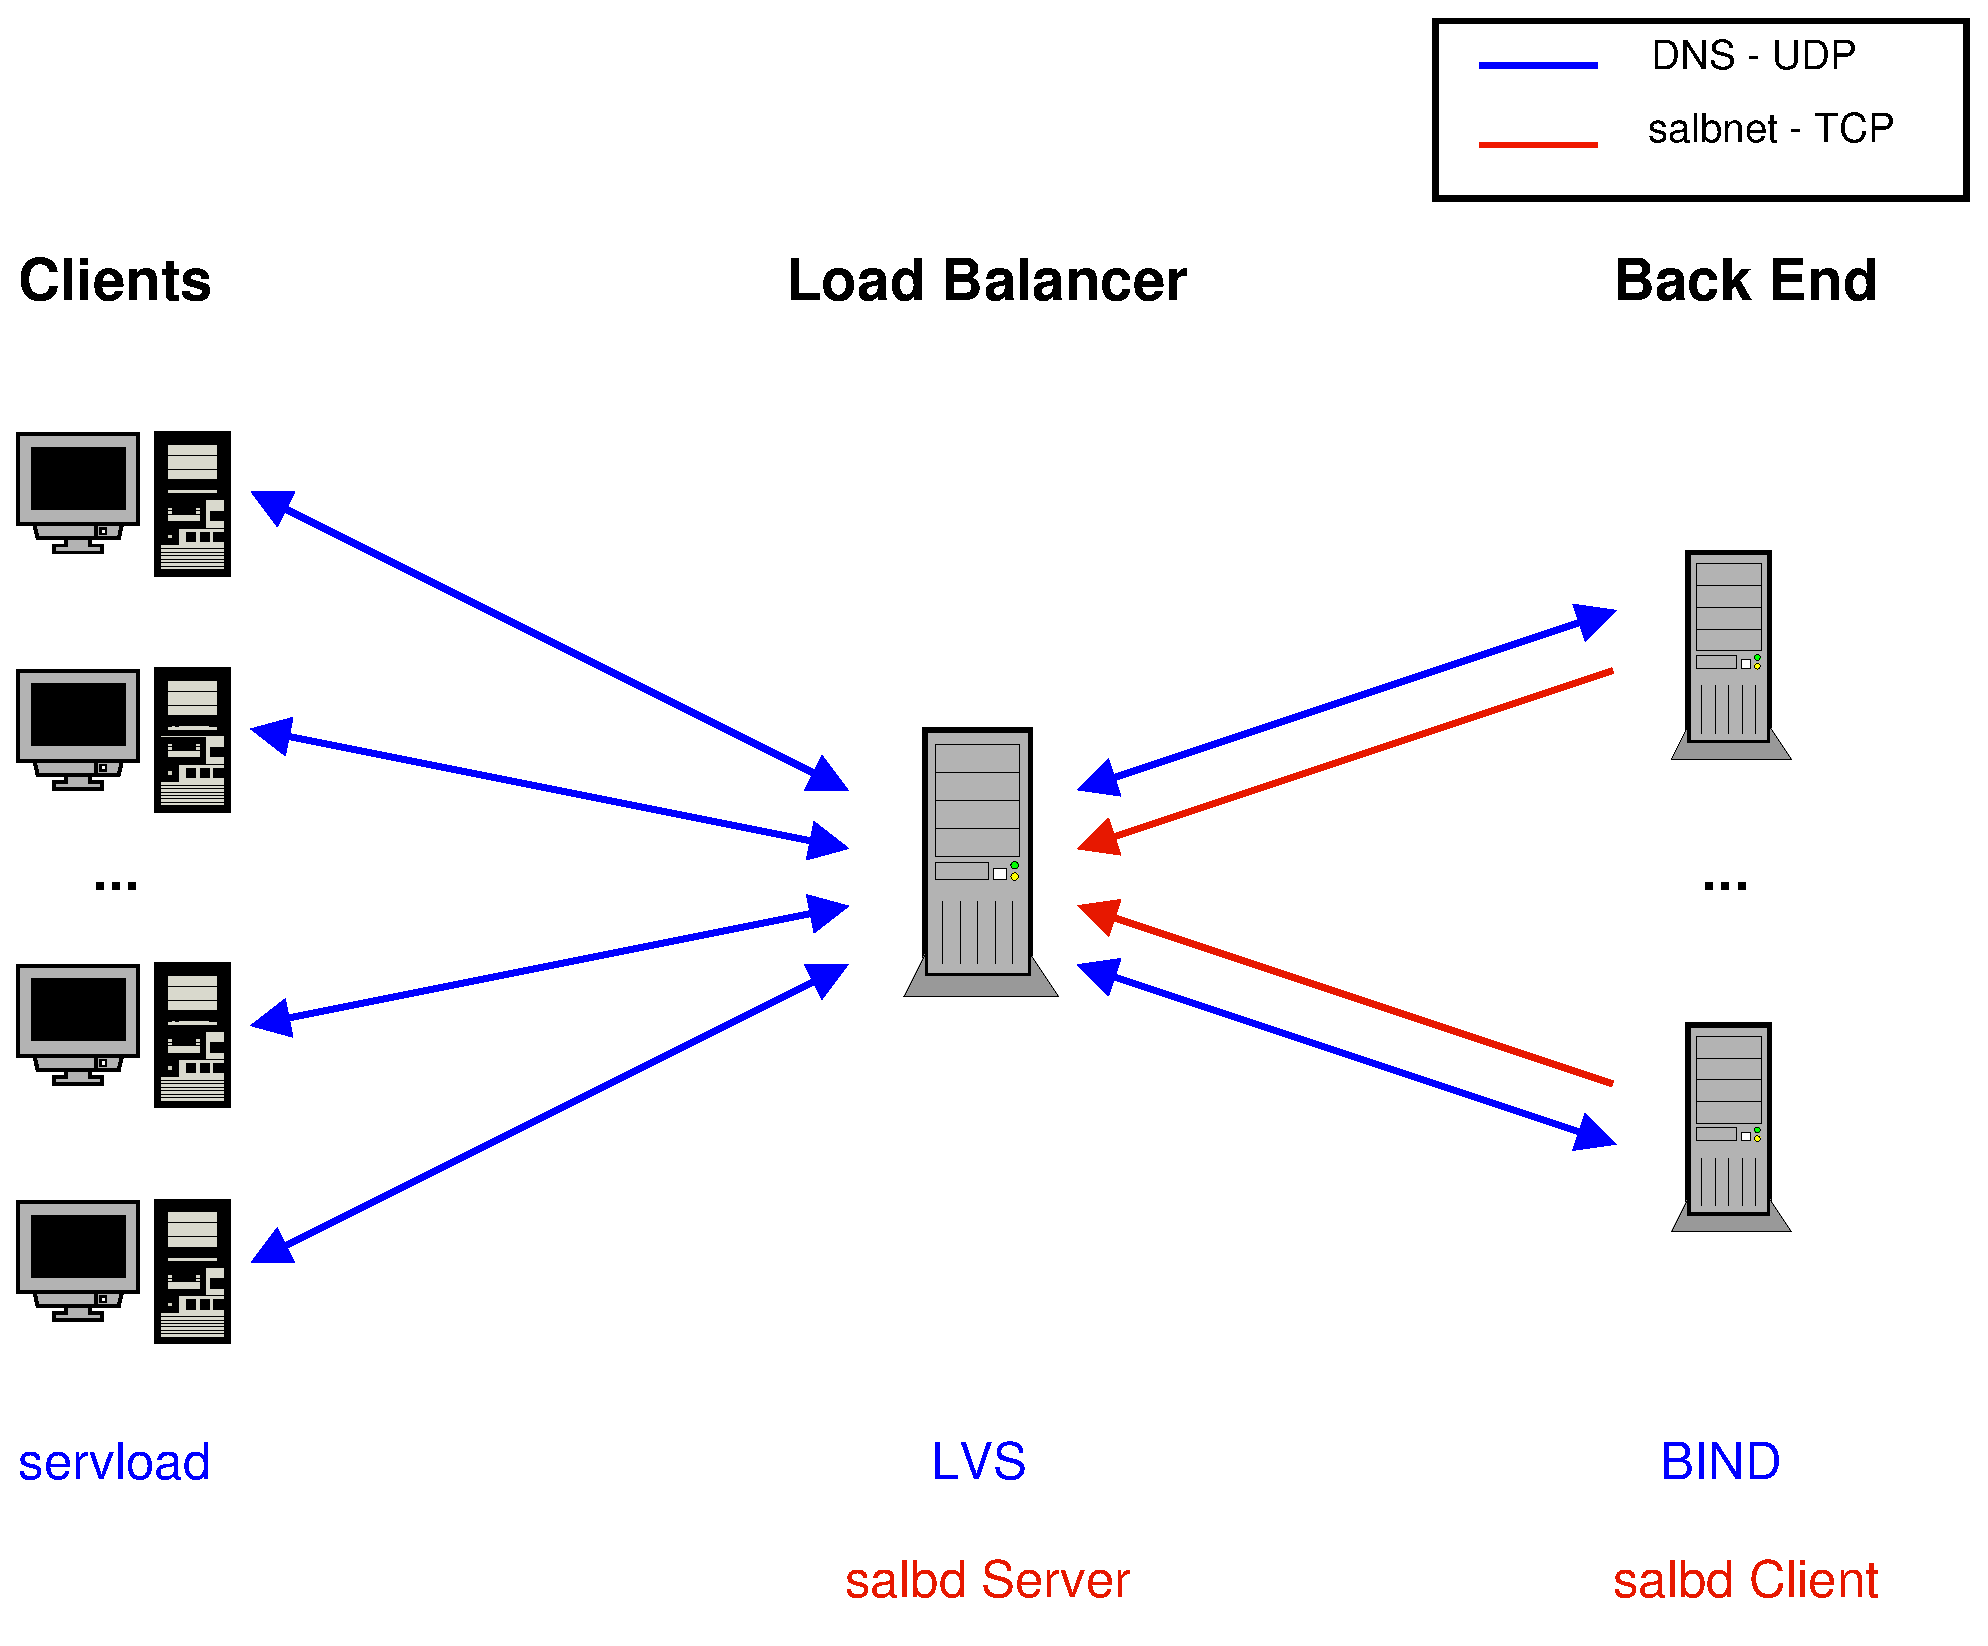
\includegraphics[scale=0.25]{images/salbd}
      \caption{servload/salbd Umgebung}
      \label{fig:images/salb}
    \end{figure}
  }

  \myframe[Aufgabenstellung]{
    \begin{itemize}
      \item Erweiterung von servload/servprep \cite{habensch}
      \item Erweiterung vom salbd Client
      \item Bestimmung von Credits auf DNS-Server für salbnet \cite{silbnet}
      \item Messungen als Funktionstest
    \end{itemize}
  }

  \mysection{DNS \cite{dnsandbind} \cite{rfc1034} \cite{rfc1035}}
  \myframe{
    \begin{itemize}
      \item Problem:
        \begin{itemize}
            \item Menschen können sich Namen gut merken
            \item Maschinen können mit Zahlen besser umgehen
        \end{itemize}
      \item Lösung: Abbildung von Namen auf Zahlen
      \item Am Anfang: ARPAnet, HOSTS.TXT, /etc/hosts
      \item Verteilte Datenbank
      \item Delegation möglich
      \item Replikation (Master/Slave), Caching
      \item Hierarchischer Namensraum (Vermeidung von Namenskonflikten)
    \end{itemize}
  }

  \myframe{
    \begin{figure}[htb!]
    \centering
    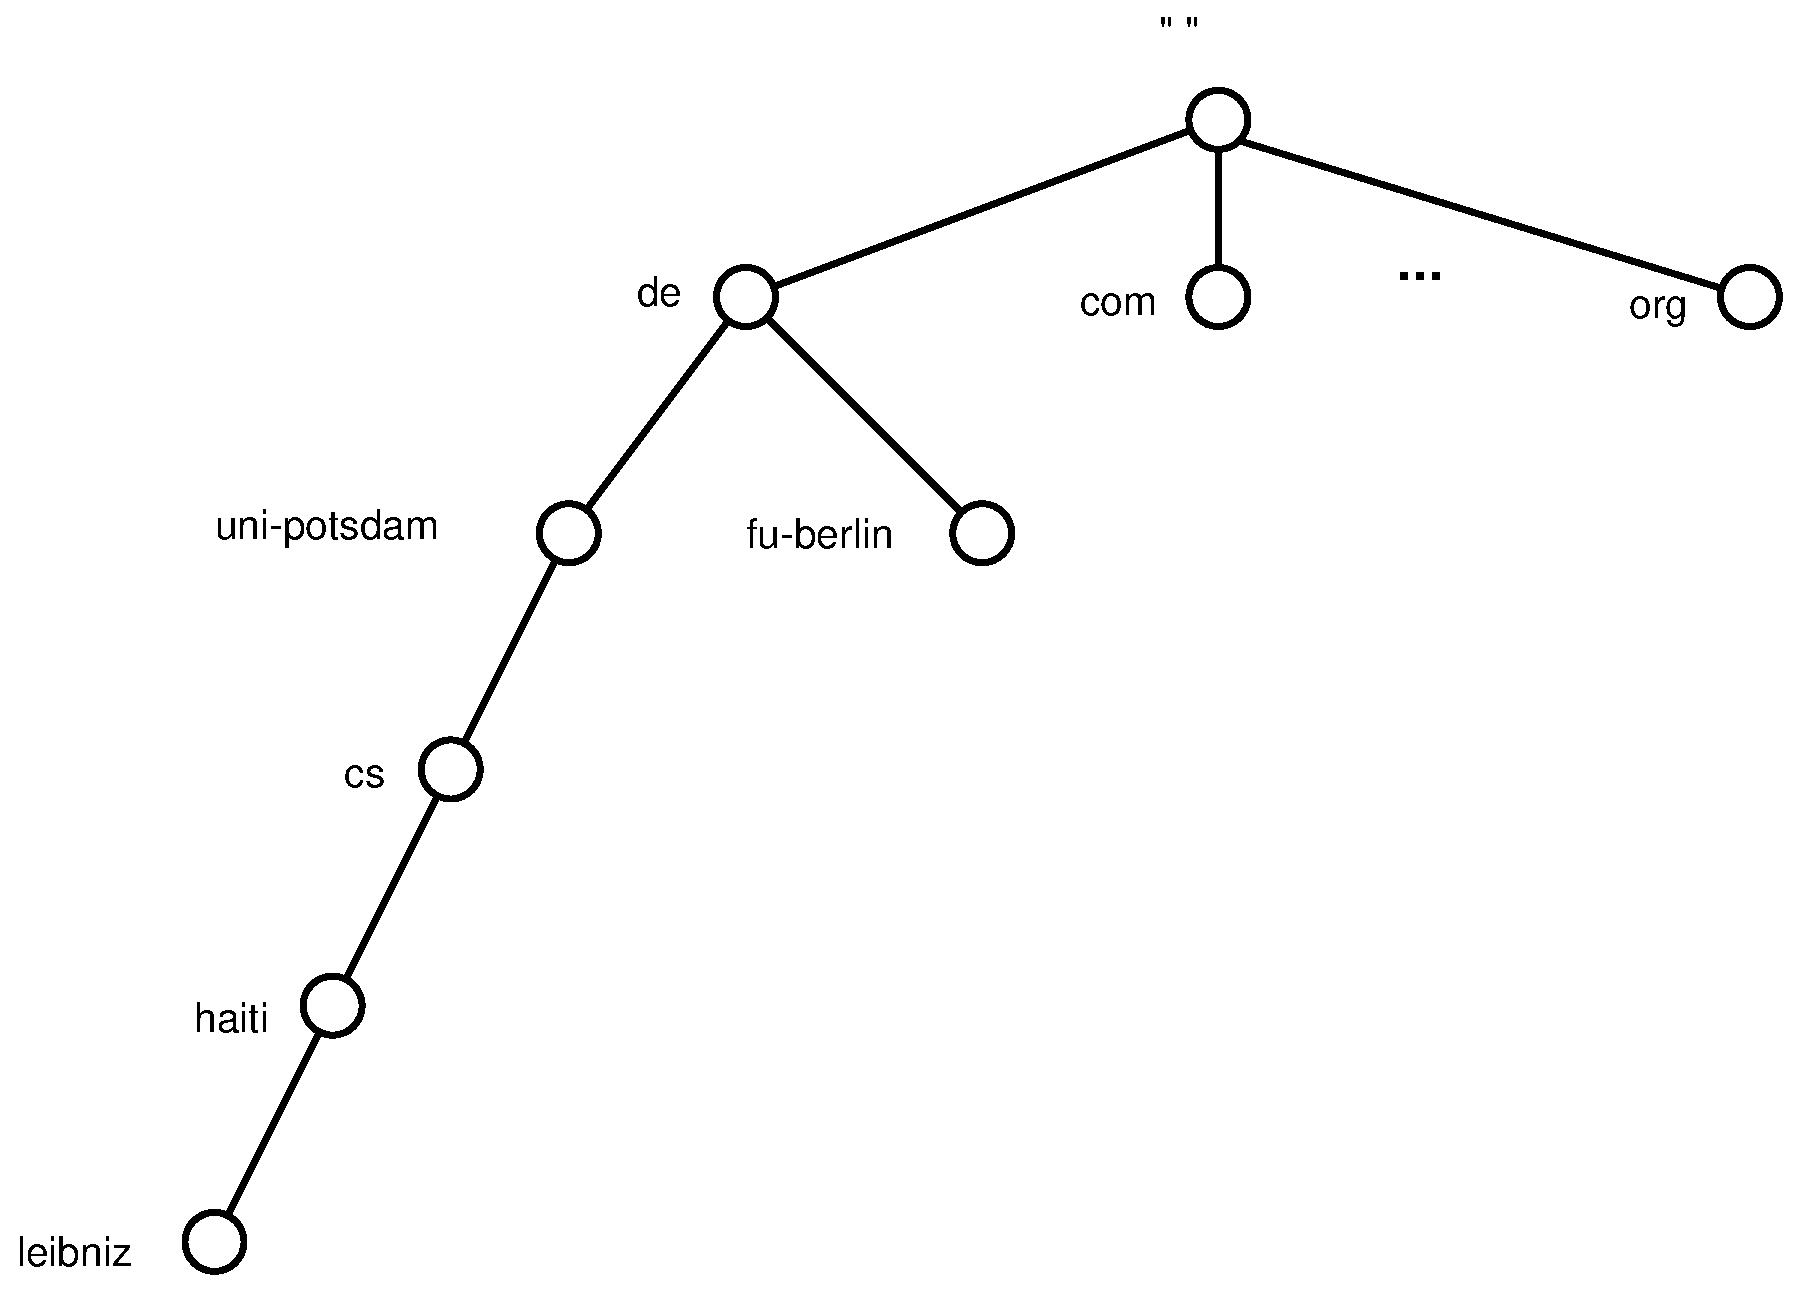
\includegraphics[scale=0.25]{images/dns-tree}
    \caption{Domain-Namensraum}
    \label{fig:images/dns-tree}
    \end{figure}
  }

  \myframe{
    \begin{figure}[htb!]
    \centering
    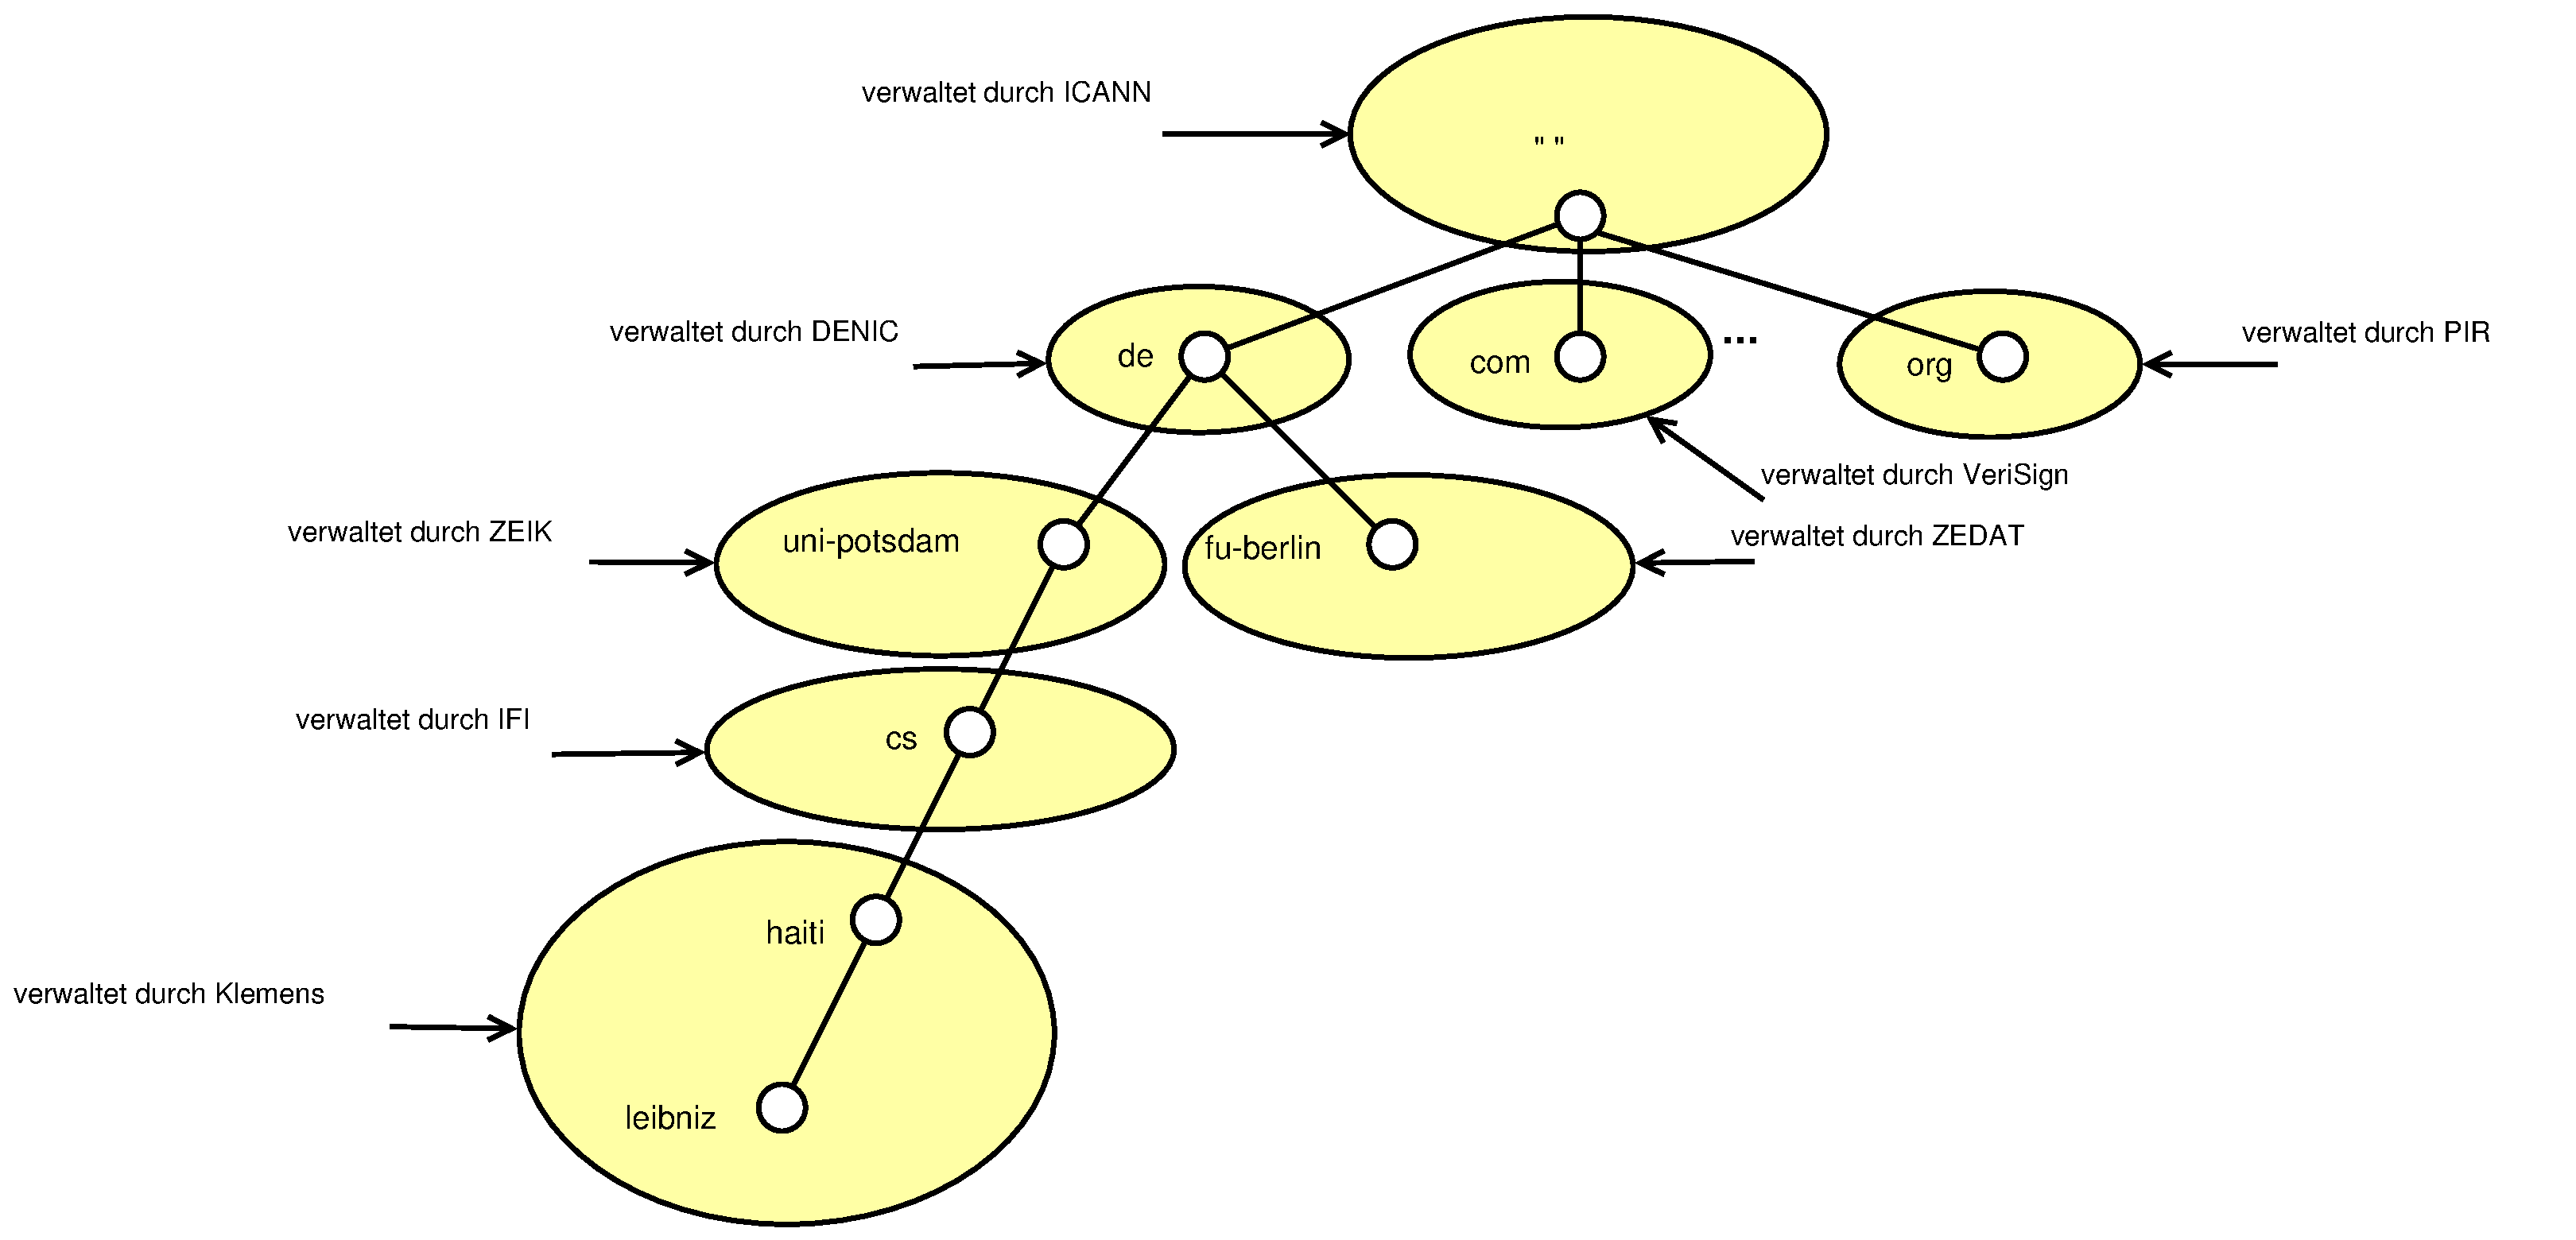
\includegraphics[width=\textwidth]{images/dns-tree2}
    \caption{Domain-Namensraum (Verantwortung)}
    \label{fig:images/dns-tree}
    \end{figure}
  }

  \myframe[Aufbau]{
    \begin{itemize}
      \item 13 root DNS-Server ([a-m].root-servers.net)\footnote{Siehe http://www.root-servers.org}
      \item 310 TLD (Stand 23.11.2011)\footnote{Siehe http://data.iana.org/TLD/tlds-alpha-by-domain.txt}
      \item SLD und ccSLD
      \item Lokale Domains
    \end{itemize}
  }

  \myframe[Einteilungen]{
    Arten von Nameservern:
    \begin{description}
        \item[Master:] lädt Zone-Daten aus einer lokalen Dateien
        \item[Slave:] erhält Zone-Daten von einem anderen Server
    \end{description}
    Arten von Abfragen:
    \begin{description}
        \item[rekursiv:]
          \begin{itemize}
              \item Nameserver soll Antwort liefern
              \item Rekursive Abfrage des Nameserver bis zum Ziel
          \end{itemize}
          \item[iterativ:] Nameserver liefert aktuell nächste Antwort
    \end{description}
  }

  \myframe[Beispiel Request]{
    \begin{figure}[htb!]
    \centering
    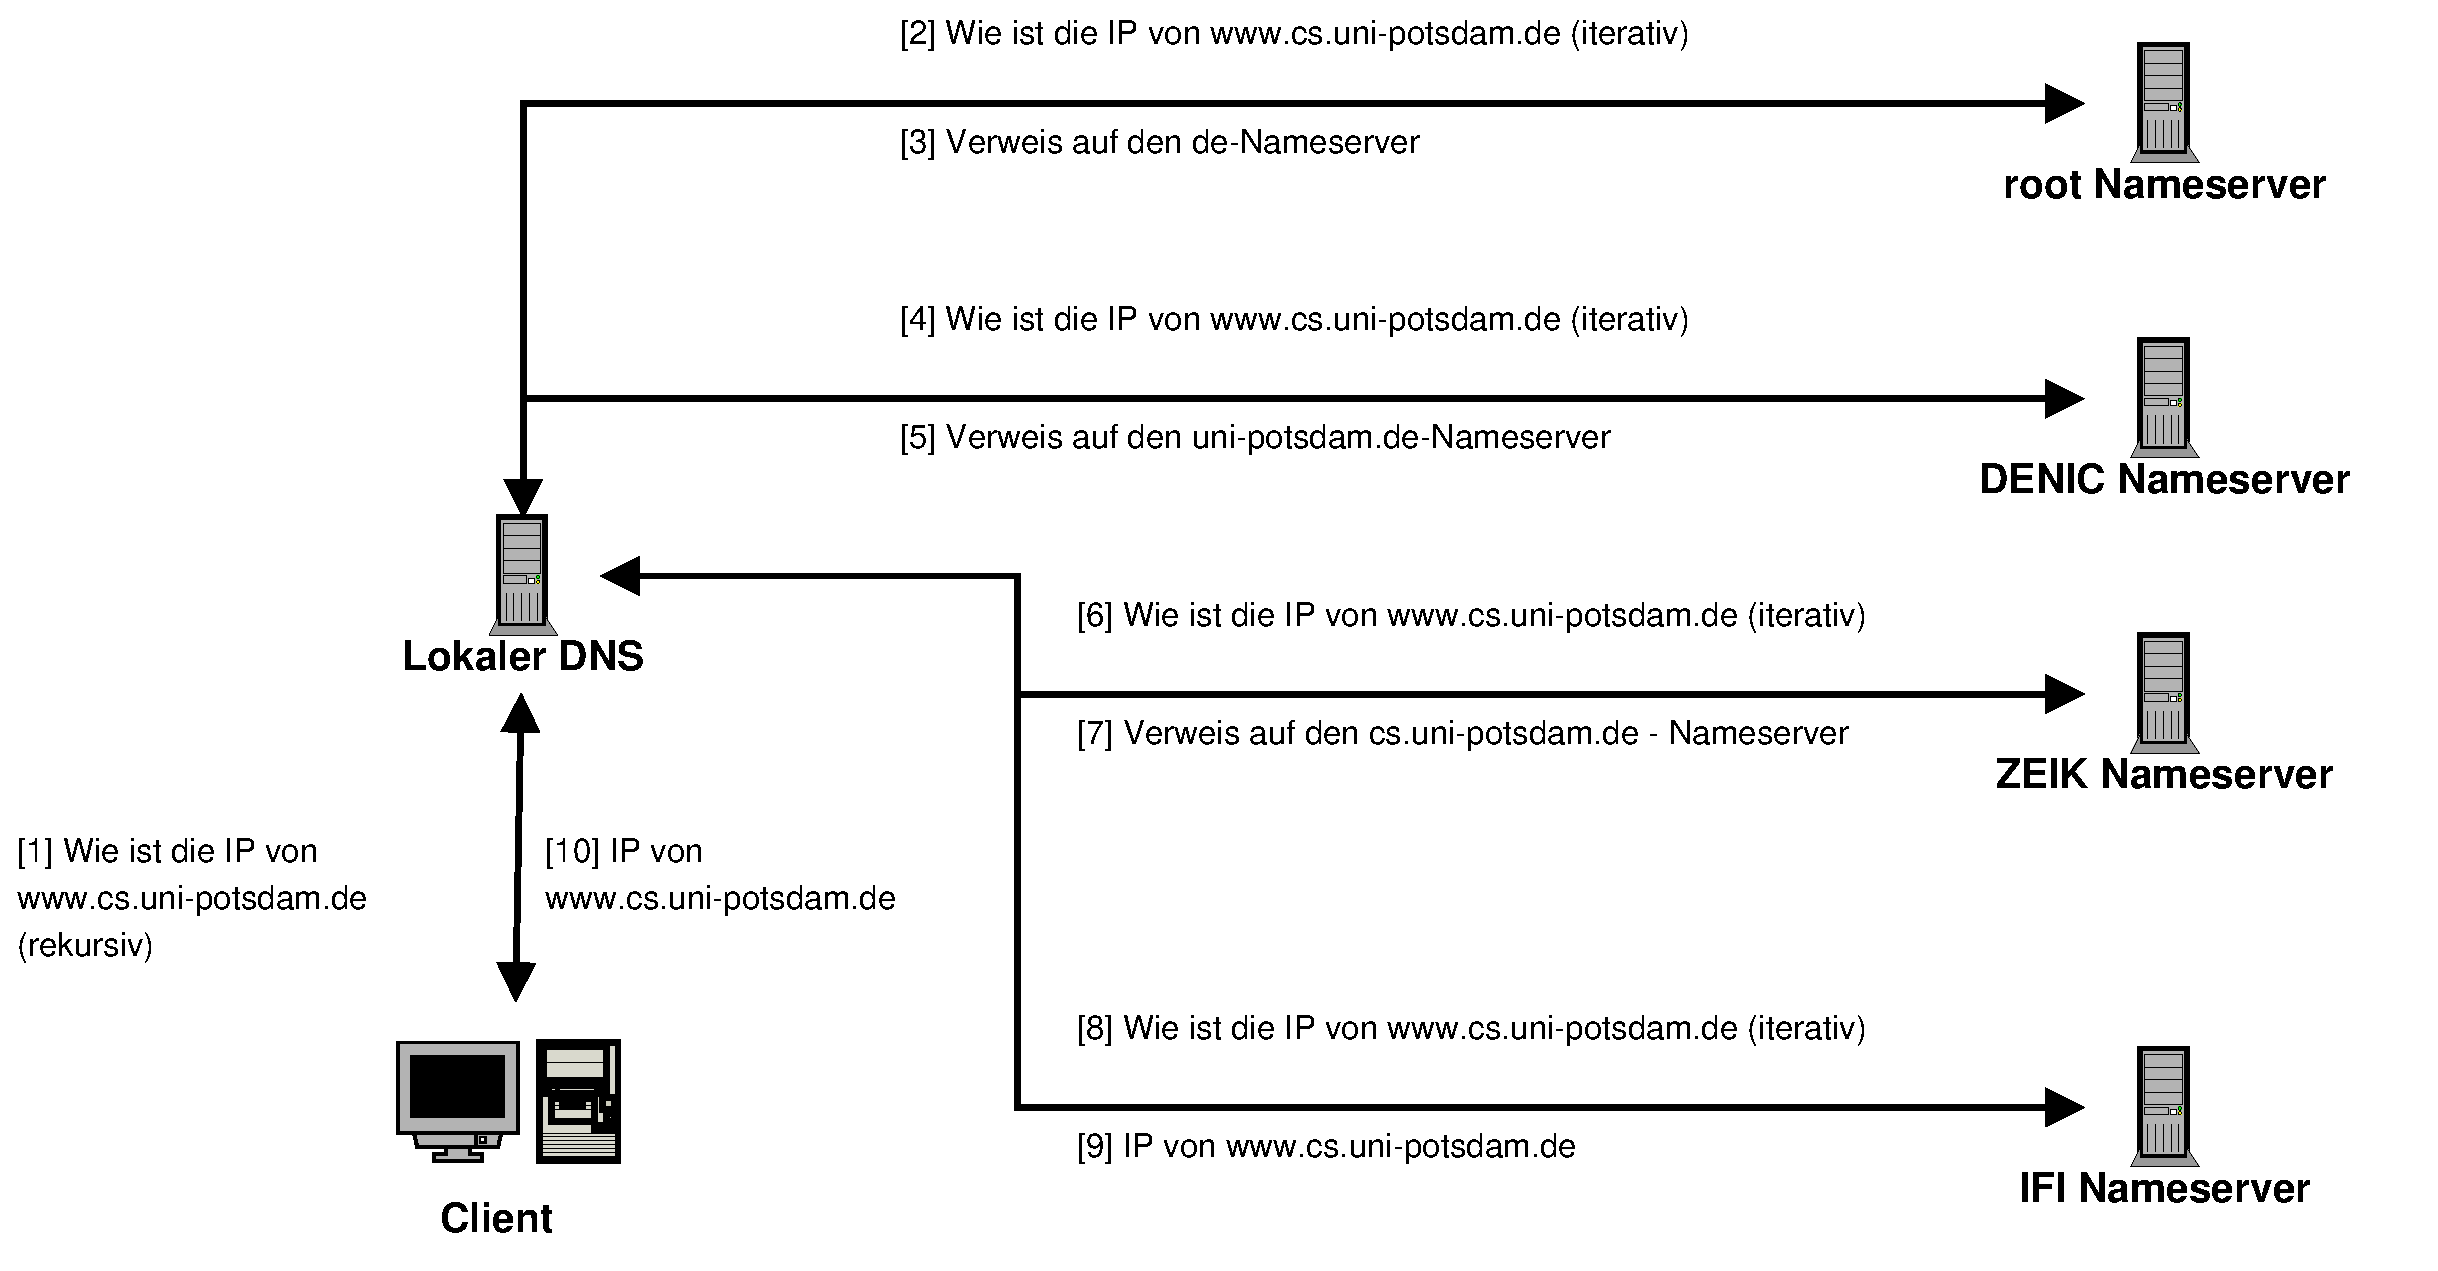
\includegraphics[scale=0.25]{images/request}
    \caption{Beispiel Request von "www.cs.uni-potsdam.de"}
    \label{fig:images/request}
    \end{figure}
  }

  \mysection{Lastverteilung}

  \myframe[Server Load Balancing] {
    Vorgehen:
    \begin{itemize}
        \item Ein Load Balancer vor mehreren Back End Server (z.B. LVS)
        \item Verschiedene Algorithmen zur Verteilung der Anfragen (Round Robin, Least Connection)
        \item Teilweise können Algorithmen mit Gewichten angepasst werden
    \end{itemize}
    Probleme:
    \begin{itemize}
        \item Ohne Gewichte wird keine Aussage über die aktuelle Last der Back End Server getroffen
        \item Korrekte Gewichte sind schwer zu bestimmen
        \item Falsche Gewichte können Situation verschlimmern
    \end{itemize}
    salbnet:
    \begin{itemize}
        \item Selbst-adaptive Lastverteilung
        \item Bisher nur Simulatormessungen
    \end{itemize}
  }

  \myframe[Standard DNS]{
    Vorgehen:
    \begin{itemize}
        \item Konfiguration von mehrere Adressen
        \item Round Robin oder Random
    \end{itemize}
    \begin{tabular}{|llll|}\hline
      www.example.com. & IN & A & 192.168.1.10 \\
      & IN & A & 192.168.1.11 \\
      & IN & A & 192.168.1.12 \\
      & IN & A & 192.168.1.13 \\\hline
    \end{tabular}
    \\~\\Probleme:
    \begin{itemize}
        \item Caching
        \item Keine Beachtung der realen Last
        \item Keine Gewichte
        \item Client entscheidet welche Adresse er nutzt
    \end{itemize}
  }

  \myframe[Erweitertes DNS] {
    Vorgehen:
    \begin{itemize}
      \item RFC 2782 \cite{rfc2782}: SRV record
        \item Angabe des Services und des Protokolls
        \item Angabe einer Priorität, eines Gewichts, des Ports und des Ziels
    \end{itemize}
    \begin{tabular}{|lllllll|}\hline
      \_http.\_tcp.bsp.de. & IN & SRV & 0 & 2 & 80 & www.bsp.de.\\
      & IN & SRV & 0 & 1 & 80 & www2.bsp.de.\\
      & IN & SRV & 1 & 0 & 80 & backup.bsp.de.\\\hline
    \end{tabular}
    \\~\\Probleme:
    \begin{itemize}
        \item Muss vom Client implementiert werden
        \item Keine Aussage ob Server erreichbar sind
    \end{itemize}
  }

  \myframe[Global Server Load Balancing (GSLB)]{
    Vorgehen:
    \begin{itemize}
        \item Load Balancer mit DNS Funktionalität
        \item Verändert originale DNS-Antwort
        \item Faktoren: Last, Response Time, Geographische Lage etc.
    \end{itemize}
    Probleme:
    \begin{itemize}
        \item Client und Lokaler DNS-Server können sehr weit entfernt sein
        \item Caching
    \end{itemize}
  }

  \myframe[Anycast]{
    Vorgehen:
    \begin{itemize}
        \item Bekanntgabe einer Anycast Adresse
        \item Server mit kürzester Route antwortet zuerst
    \end{itemize}
    Verwendung:
    \begin{itemize}
        \item Viele root DNS-Server sind über mehrere Kontinente verteilt
        \item Für diese root DNS-Server ist eine Anycast Adresse bekannt
    \end{itemize}
  }

  \myframe[Anycast] {
    \begin{figure}[htb!]
    \centering
    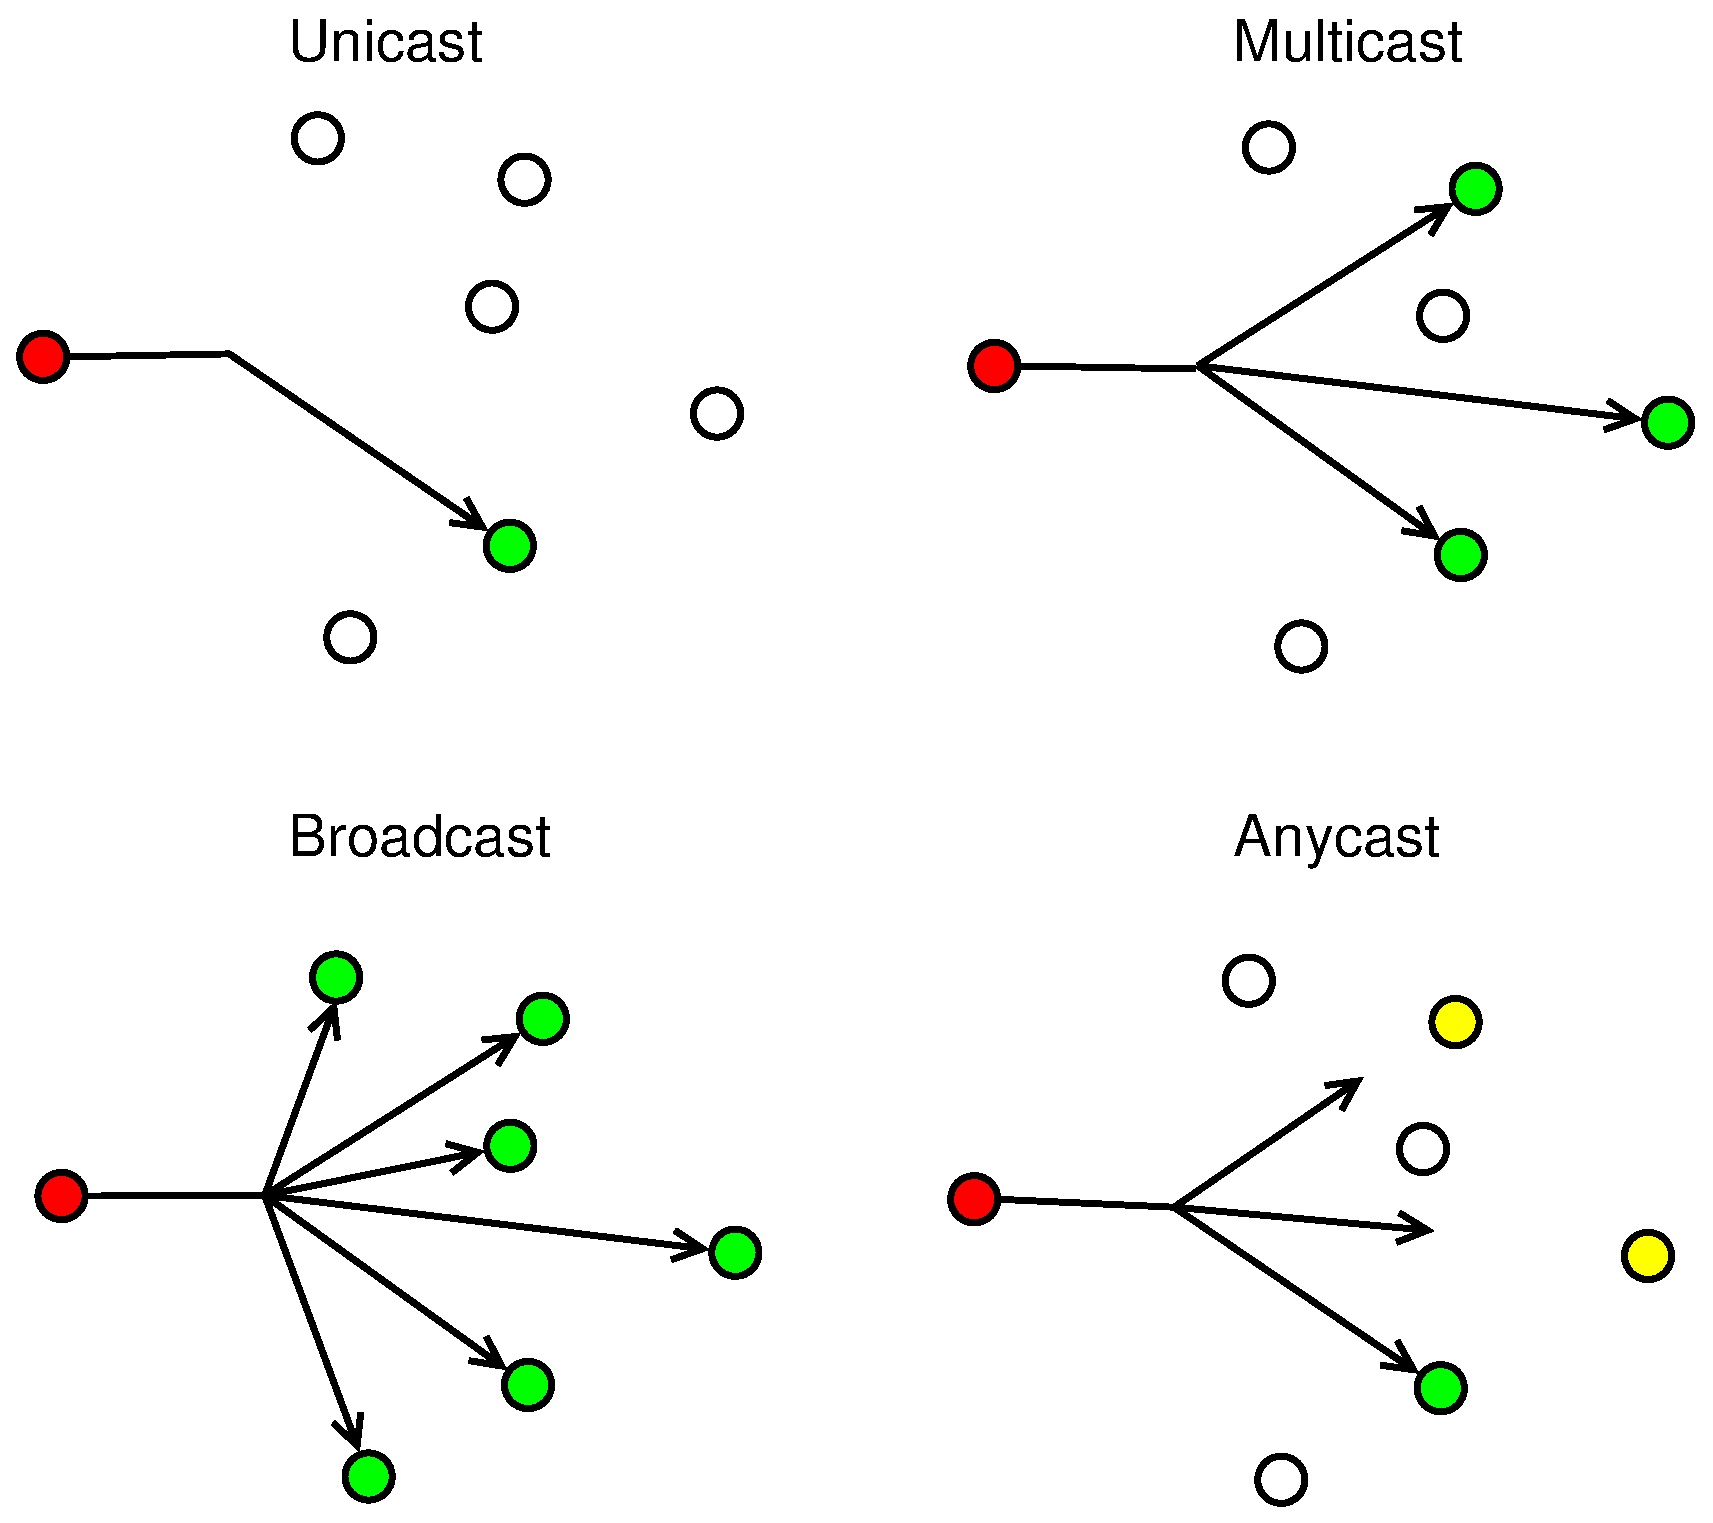
\includegraphics[scale=0.25]{images/cast}
    \caption{Übersicht Adressierungsarten}
    \label{fig:cast}
    \end{figure}
  }

  \mysection{Einordnung}

  \myframe[DNS Lastverteilung Einordnung]{
    \begin{description}
      \item[Root Server:] Anycast/DNS Cluster
      \item[TLD:] Anycast/DNS Cluster
      \item[Firmen:] DNS Cluster/DNS LB
      \item[Lokal:] DNS LB
    \end{description}
  }

  \myframe[Ziel]{
    \begin{figure}[htb!]
      \centering
      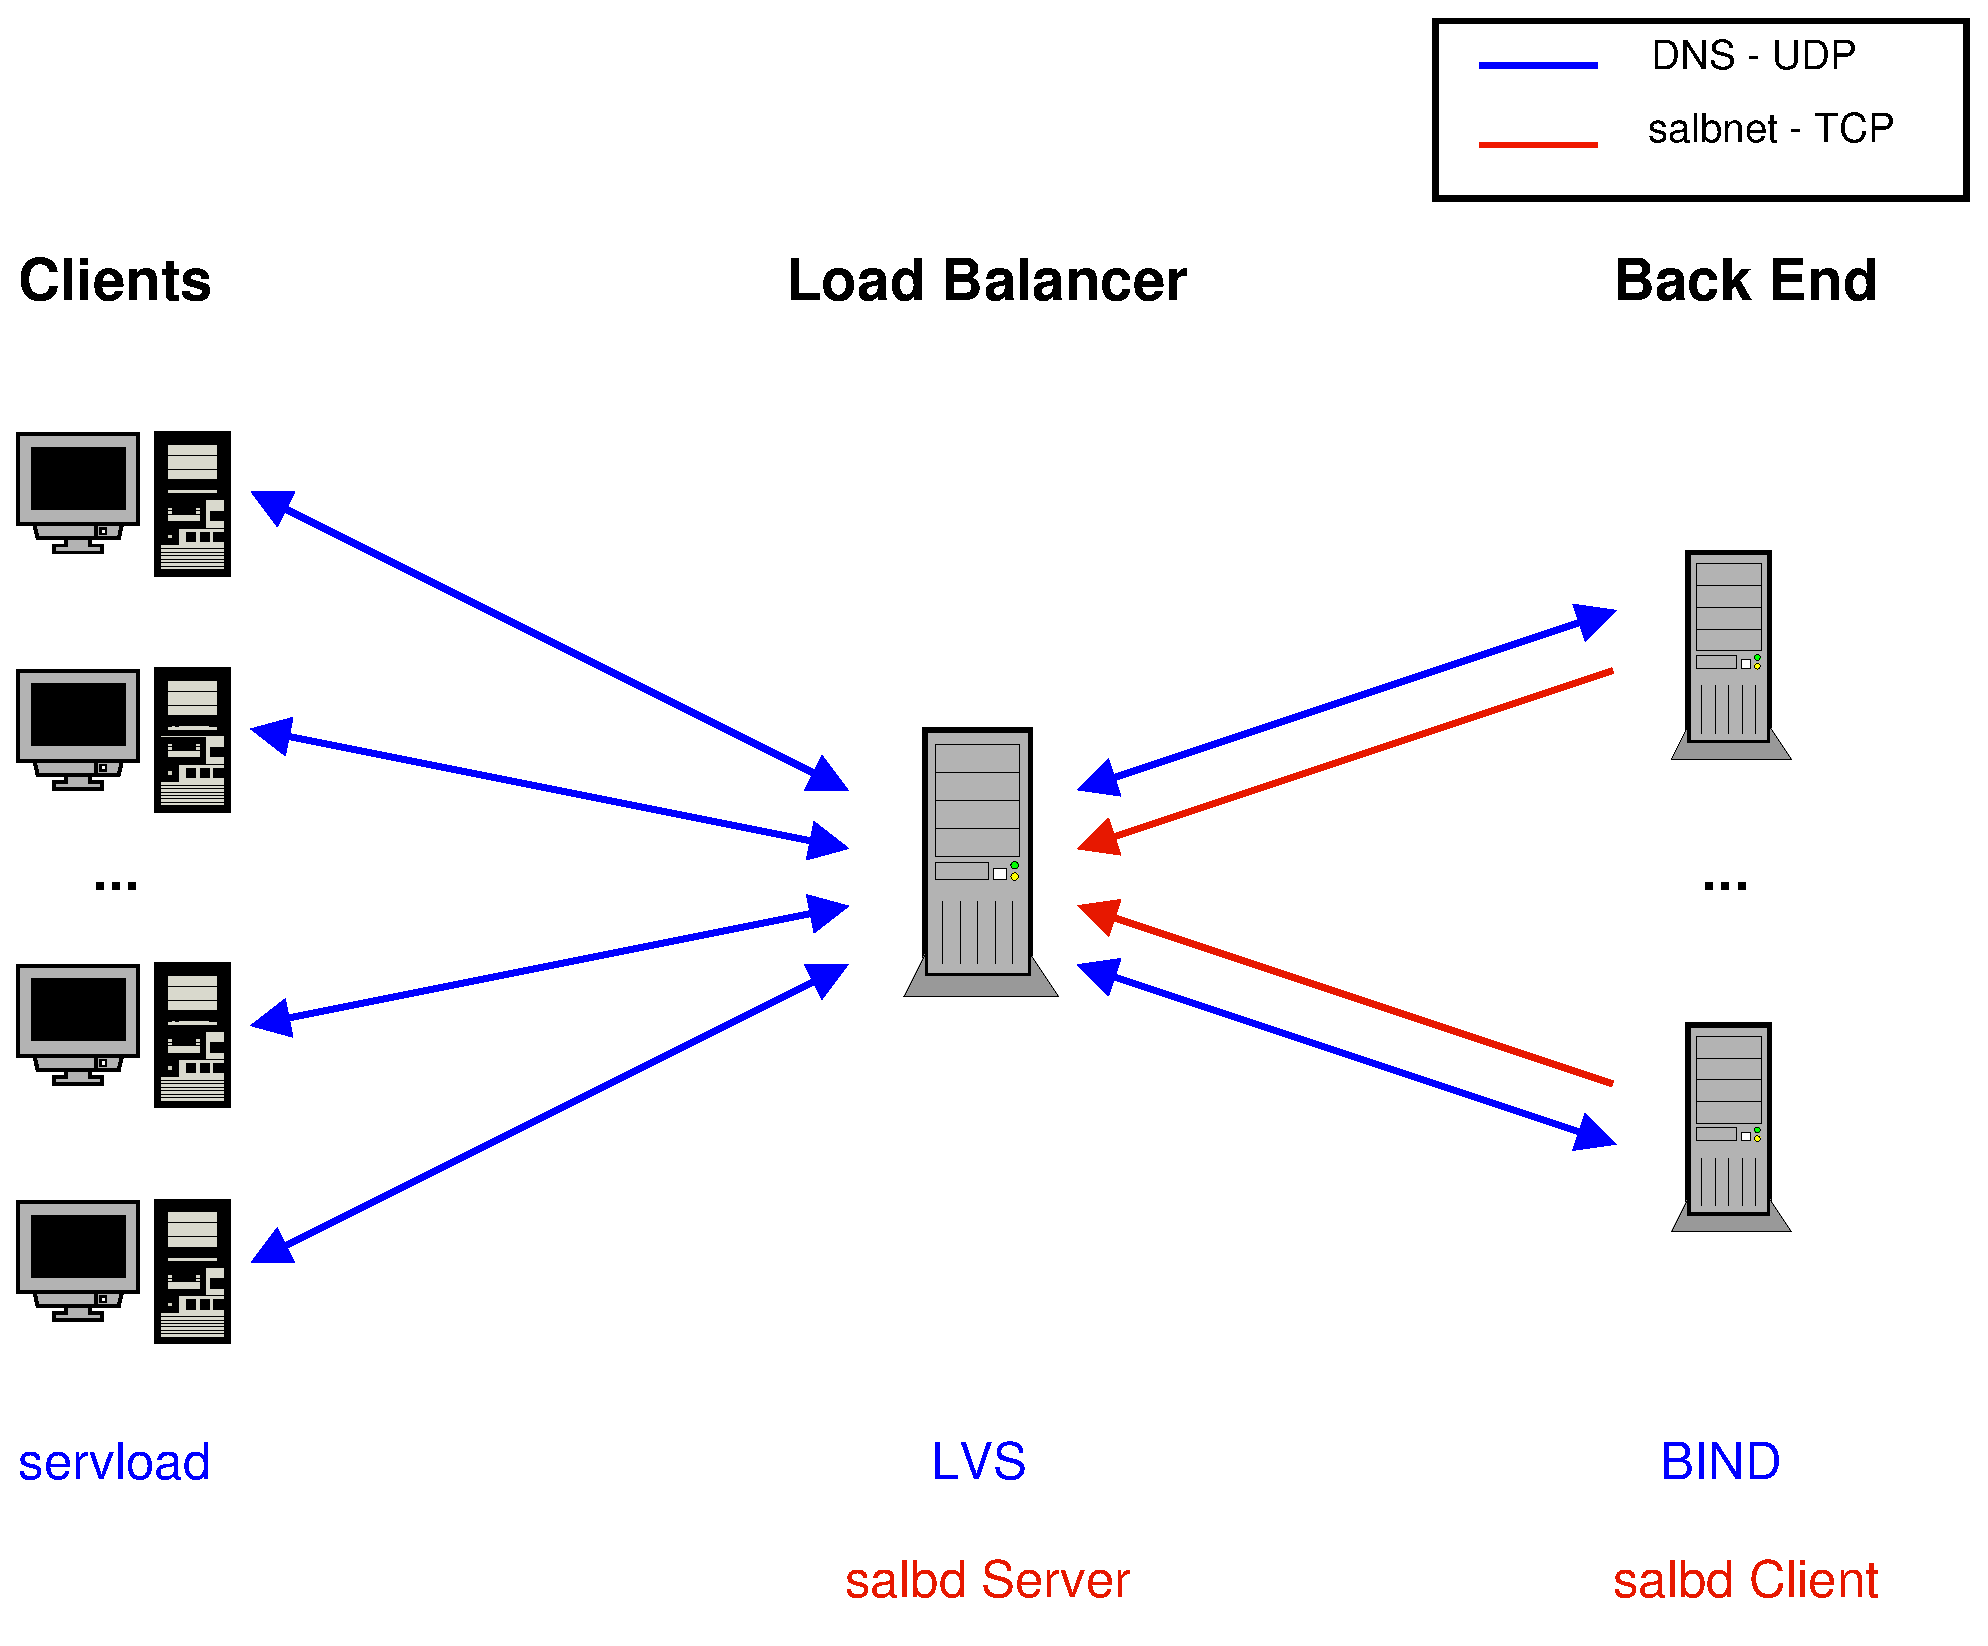
\includegraphics[scale=0.25]{images/salbd}
      \caption{servload/salbd Umgebung}
      \label{fig:images/salb}
    \end{figure}
  }


  \appendix{}
  \newcounter{finalframe}
  \setcounter{finalframe}{\value{framenumber}}
  \pagestyle{empty}
  \renewcommand{\mytitle}{Literaturverzeichnis}
  \frame[allowframebreaks]{\frametitle{\mytitle}
   \bibliographystyle{gerplain}
    \bibliography{references}
  }
  \setcounter{framenumber}{\value{finalframe}}

\end{document}

%%% Local Variables: 
%%% mode: latex
%%% TeX-master: t
%%% End: 
